\chapter{Fundamentação}
    \label{chap:fundamentacao}
    
    Este capítulo apresenta os fundamentos necessários para o entendimento do desenvolvimento do trabalho. As duas primeiras seções abordam os conceitos de tempo real e DVFS utilizados. A terceira e última seção aborda estes dois primeiros conceitos somados, apresentando então a ideia de DVFS em tempo real.
    
    \section{Sistema de Tempo Real}
        \label{sec:sistema-de-tempo-real}
        
        Esta seção apresenta o modelo de sistema de tempo real que será utilizado neste trabalho. Ele é baseado diretamente no modelo que \citeonline{Pillai:2001} utilizam para propor as heurísticas escolhidas para implementação. Neste cenário, um sistema de tempo real é um conjunto de tarefas periódicas com prazos definidos, todas concorrendo por um único processador. Ainda, para os efeitos deste trabalho, as tarefas apresentadas são passíveis de preempção, ou seja, a qualquer momento podem ser interrompidas para que cedam o uso processador.
    
        \subsection{Modelo de Sistema de Tempo Real}
            \label{sec:modelo-de-sistema-de-tempo-real}
    
        No modelo em questão, o sistema é composto por um conjunto de tarefas periódicas que não compartilham nenhum recurso entre si. Assim sendo, a toda tarefa $T_i$, tem-se atribuído um \emph{período} $P_i$, de modo que a tarefa $T_i$ sempre é \emph{requisitada} para execução a cada $P_i$ unidades de tempo. Observe que mesmo sendo requisitada no início de cada período, a tarefa pode iniciar sua execução efetiva a qualquer momento dentro do período, devido, por exemplo, a uma outra tarefa de maior prioridade estar ocupando o processador.
        
        Denomina-se \emph{tempo de resposta} o tempo entre a requisição e a conclusão da tarefa. Neste trabalho, assume-se que para efeitos de estabilidade do sistema, o tempo de resposta de uma tarefa nunca deve exceder seu respectivo período. Neste sentido, se uma tarefa $T_i$ começa a ser executada entre os tempos $t$ e $t+P_i$, sua conclusão não deve exceder $t+P_i$, sendo este limite também chamado de \emph{deadline}.
        
        Como pode-se esperar em um sistema comum, cada execução de $T_i$ pode possuir um tempo de resposta diferente. Para que o escalonador de tarefas de tempo real seja capaz de ordenar múltiplas tarefas de modo que estas não ultrapassem seus deadlines, este modelo também utiliza o \emph{pior tempo de computação} $C_i$ associado à tarefa $T_i$, ou seja, toda tarefa que é iniciada em $t$, caso ela nunca deixe o processador, sempre tem sua conclusão antes ou exatamente no momento $t+C_i$. Finalmente, a figura \ref{fig:exemplo-de-aplicacao} exemplifica este modelo com um sistema composto por duas tarefas $T_1$ e $T_2$ sendo executadas.
        
        \begin{center}
    	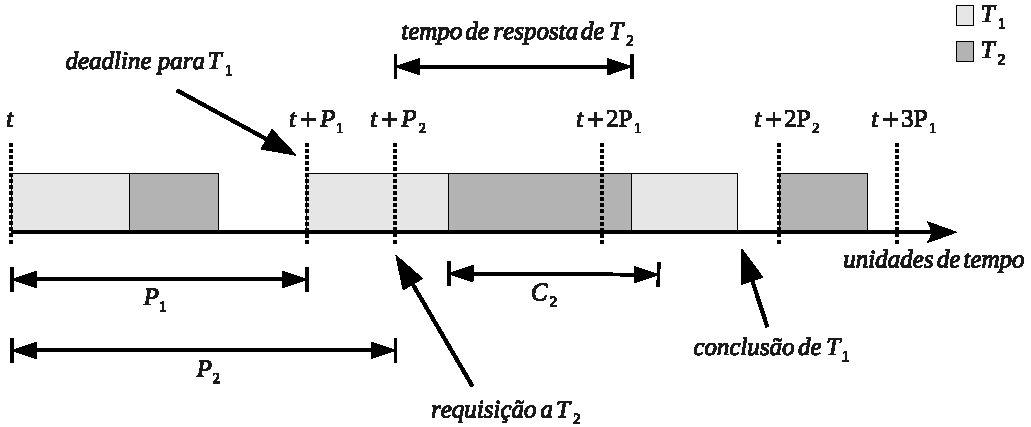
\includegraphics[scale=0.8]{imagens/exemplo-sistema-de-tempo-real.pdf}
        \captionof{figure}{Exemplo do modelo de sistema de tempo real utilizado}
	    \label{fig:exemplo-de-aplicacao}
        \end{center}
        
        Dado o modelo apresentado, é possível definir a \emph{utilização} $U_i$ de uma tarefa $T_i$ em um único processador como sendo $U_i = C_i/P_i$. Diz-se que a \emph{utilização total} por um conjunto de $n$ tarefas $T_i$ é, então, $$U = \sum_{i=1}^{n}\frac{C_i}{P_i}.$$
        
        Pode-se supor que a troca de contexto entre tarefas de uma aplicação dá-se através de uma rotina em software. Obviamente esta rotina também ocupa tempo de processamento no sistema, mas esta faixa de tempo pode ser negligenciada no modelo, pois é possível tratá-la como parte do pior tempo de computação das tarefas em execução.
            
    \subsection{Escalonador de Tempo-Real}
        \label{sec:escalonadores}
    
        Um sistema operacional de tempo real, também chamado de RTOS (\emph{Real-Time Operating System}), é o programa de computador que, além de atender a outras responsabilidades, ordena a execução de tarefas da aplicação de modo a responder em tempo hábil alguma requisição. Mais detalhadamente, o componente do RTOS responsável por esta ordenação é o \emph{escalonador de tempo real} \cite{Li:2003,Pillai:2001}. É este componente que deve prover um ou mais algoritmos que resolvem as prioridades de execução das tarefas do sistema, a fim de que nenhuma delas perca seu deadline.
        
        Para que o escalonador de tempo real seja capaz de garantir a execução em tempo hábil de um conjunto de tarefas, duas condições são estabelecidas:
        
        \begin{itemize}
        	\item O conjunto de tarefas deve ser \emph{escalonável}. Isto significa que o conjunto de tarefas deve passar por um ou mais testes propostos pelo algoritmo do escalonador, justamente para que este conjunto satisfaça as premissas de modo que o algoritmo mantenha suas propriedades. Estes testes são chamados de \emph{testes de escalonabilidade}.
        	\item Nenhuma das tarefas excede seu pior tempo de computação (como elaborado na seção \ref{sec:modelo-de-sistema-de-tempo-real}).
        \end{itemize}
        
        Ainda quanto à ordenação realizada pelo escalonador, esta pode ser entendida como a atribuição de uma prioridade a cada tarefa. Essa atribuição pode ser realizada durante a execução ou previamente. Quando as prioridades são decididas durante execução, diz-se que o escalonador ou o escalonamento é \emph{dinâmico}. No caso em que as prioridades são atribuídas anteriormente à execução, diz-se que o escalonador ou o escalonamento é \emph{estático}.
        
        Quando um escalonador pode interromper a execução de uma tarefa para que uma de maior prioridade ganhe o processador, diz-se que este é um \emph{escalonador preemptivo}.
        
        Dentre os algoritmos para escalonadores de tempo real existentes, este trabalho utiliza o \emph{Earliest Deadline First}, ou simplesmente EDF. Usualmente, diz-se então que o escalonamento ou escalonador utilizado é EDF, e é nele que a heurística \emph{Cycle-conserving RT-DVS} para EDF se baseia. O mecanismo de ordenação do algoritmo EDF é explicado na subseção seguinte (\ref{sec:edf}).
                   
    \subsection{Escalonador \emph{Earliest Deadline First}}
        \label{sec:edf}
        
        O algoritmo \emph{Earliest Deadline First} é um algoritmo para escalonamento dinâmico. Seu funcionamento dá-se com a atribuição de prioridades às tarefas, de modo que quanto mais próxima do deadline a tarefa está, maior é sua prioridade \cite{Liu:1973}. A figura \ref{fig:exemplo-edf} demonstra um exemplo de escalonamento EDF para duas tarefas, onde cada $d_i$ representa deadlines para a tarefa $T_i$. Ambas tarefas tem sua primeira requisição em $t$. Observe que no primeiro deadline $d_1$ acontece a preempção de $T_2$, pois neste momento há uma nova requisição de $T_1$, que por sua vez apresenta um deadline mais próximo que $T_2$.
        
        \begin{center}
    	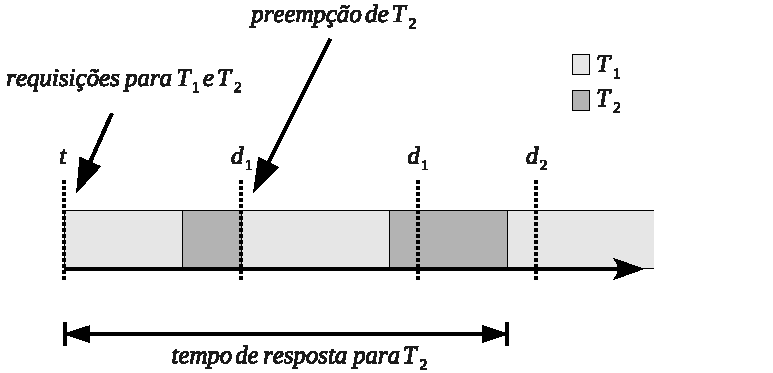
\includegraphics[scale=0.8]{imagens/exemplo-edf.pdf}
        \captionof{figure}{Exemplo de escalonamento EDF para duas tarefas}
	    \label{fig:exemplo-edf}
        \end{center}        
        
        Um teste de escalonabilidade para o EDF é o seguinte:
        
        Dado um conjunto $T$ de $n$ tarefas $T_i$, para $1 \leq i\leq n$, tais que:

   	    \begin{itemize}
	        \item sejam independentes entre si;
	        \item sejam passíveis de preempção;
	        \item sejam periódicas;
	        \item possuam deadlines iguais a seus respectivos períodos.
	    \end{itemize}
        
        Então, $T$ é escalonável por um escalonador EDF se, e somente se $$ \sum_{i=1}^{n} \frac{C_i}{P_i} \leq 1.$$
        
        O teste descrito nada mais é do que a verificação da utilização total do processador para conjunto de tarefas $T$. Este teste, por si só, já é necessário e suficiente para que o conjunto de tarefas seja escalonável.
        
    \section{\emph{Dynamic Voltage and Frequency Scaling}}
    
        \emph{Dynamic Voltage and Frequency Scaling} (DVFS), ou também \emph{Dynamic Voltage Scaling} (DVS), é a capacidade ou atitude de um processador alterar sua tensão e frequência durante a execução de um programa, ou seja, alterar sua tensão e frequência dinamicamente \cite{Pillai:2001}.
        
        A ideia desta técnica é oferecer um contrato entre desempenho de processamento e consumo de energia. A fundamentação desta troca se estabelece sobre duas importantes características da tecnologia de sistemas computacionais atual: \begin{itemize} \item Primeiramente, quase a totalidade destes sistemas são baseados em lógica CMOS. \item Em segundo, o pico de computação das aplicações, sejam elas embarcadas ou não, é usado apenas durante uma pequena fração do tempo de funcionamento desses sistemas. \end{itemize}
        
        % No parágrafo anterior falta uma citação sobre CMOS
        
        A primeira característica apresentada influi no contrato, pois, pelas propriedades físicas dos circuitos CMOS atuais, a energia dissipada ($P$) é fortemente relacionada à frequência ($f$) e à tensão de funcionamento ($V$) do sistema, dois fatores fundamentais para o desempenho \cite{Snowdown:2005}. Esta proporção é visível da seguinte forma: $$P \propto fV^2.$$
        
        Levando em conta que o tempo de computação é inversamente proporcional a $f$, pode-se dizer que a energia $E$, utilizada na computação de uma tarefa em um processador CMOS, é estabelecida conforme a seguinte proporção: $$E \propto V^2.$$ 
        
        Detalhando esta primeira característica, diminuindo a frequência para a redução de consumo de energia, o tempo para o término da dada tarefa aumenta, ou seja, mesmo com um consumo energético menor, este consumo será mantido por mais tempo. Por outro lado, diminuindo-se a frequência, aumenta-se o período entre os chaveamentos do circuito digital, tornando o efeito temporal da capacitância mais tolerável, daí a possibilidade de redução da tensão. Mesmo que o tempo de execução da tarefa seja linearmente proporcional à frequência, a energia gasta é quadraticamente proporcional à tensão, permitindo um ganho energético. Na figura \ref{fig:dvs} um exemplo é ilustrado para uma tarefa que possui tempo de computação exato de 20 milisegundos a 20MHz. Mesmo reduzindo-se pela metade a frequência do processador, tomando-se o dobro de tempo para a execução da tarefa exemplo, ainda há redução no consumo de energia.    

        \begin{figure}
        \begin{center}
        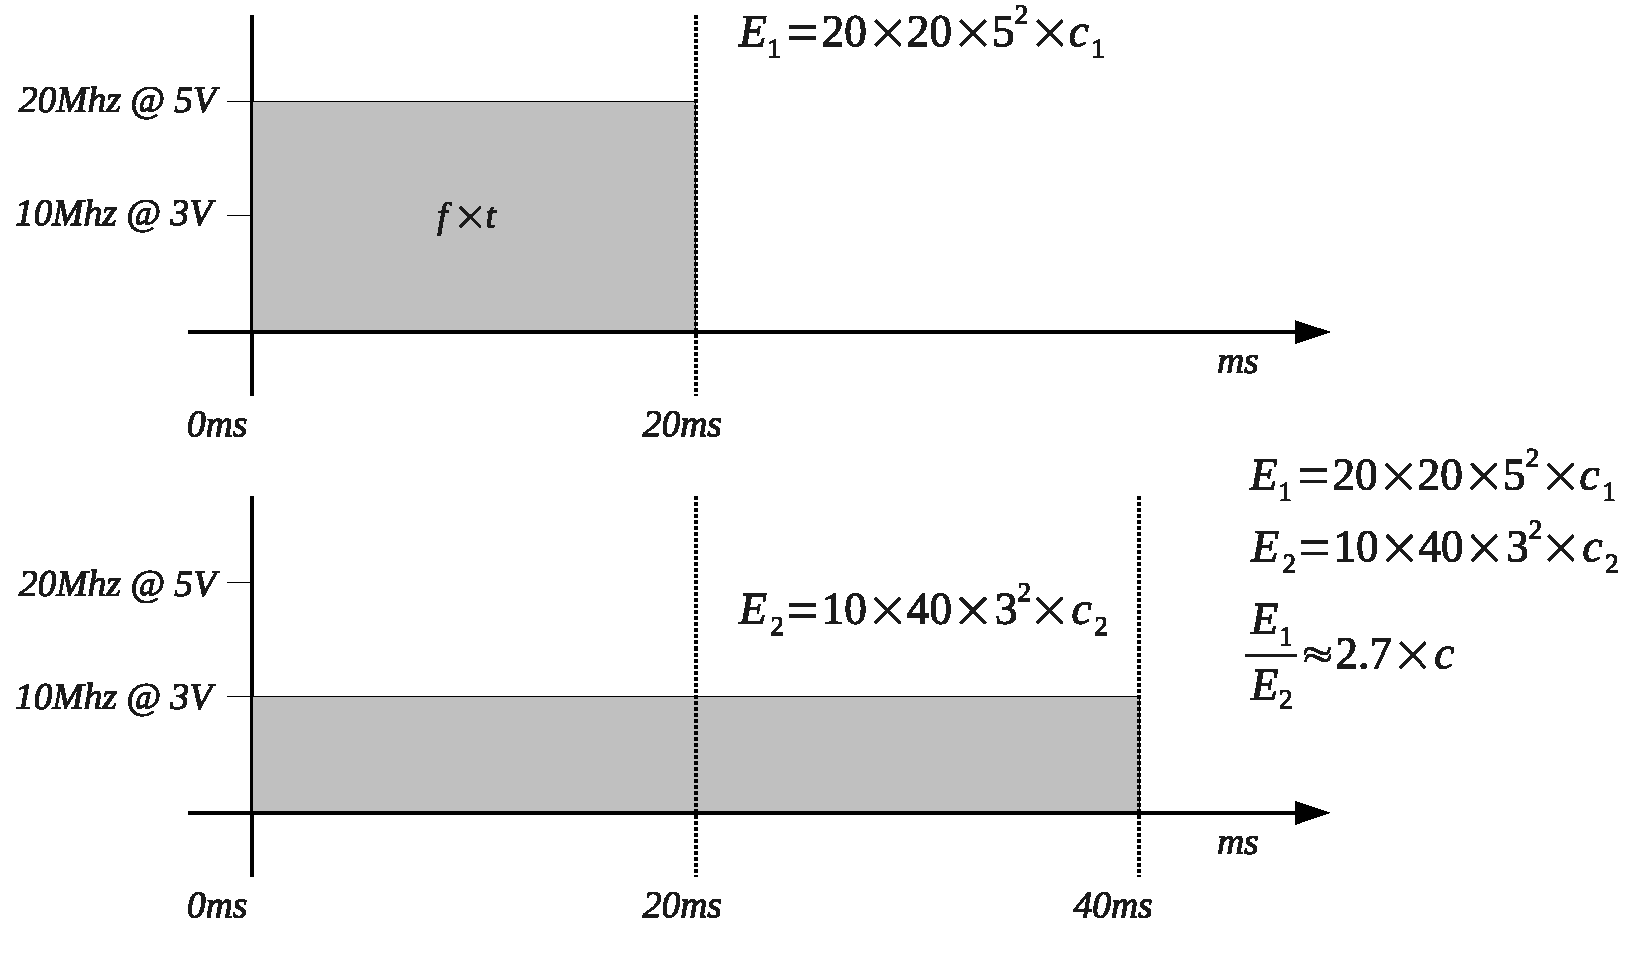
\includegraphics[scale=0.5]{imagens/exemplo-tarefas-dvs.pdf}
        \captionof{figure}{Exemplo de ganho energético obtido através de DVFS}
        \label{fig:dvs}
        \end{center}
        \end{figure}
        
        Finalmente, tendo em foco a segunda característica, que diz respeito ao pico e a média de computação necessária em um sistema computacional, pode-se então, ajustando-se a frequência às necessidades da aplicação, consumir a energia necessária para alto desempenho somente nos momentos realmente requisitados pela aplicação.
        
        Os processadores que implementam esta tecnologia oferecem uma interface que permite, ao software em execução, a alteração dinâmica da tensão. Essa interface, geralmente, é disponível na forma de registradores ou instruções especiais. Um exemplo seria a implementação Intel SpeedStep para núcleos ARM. Neste caso, expande-se a arquitetura ARM do processador através de um co-processador, o qual possui registradores acessíveis através do conjunto de instruções ARM padrão. É possível então, através destes registradores, configurar dinamicamente modos de operação não somente para o núcleo (CPU), mas também para o barramento principal e memória. Cada um destes modos de operação estabelece uma tensão e sua respectiva frequência de funcionamento para estes dispositivos \cite{Snowdown:2005}.
        
    \section{\emph{Real-Time Dynamic Voltage and Frequency Scaling}}
    
        \emph{Real-Time Dynamic Voltage (and Frequency) Scaling}, ou simplesmente RT-DVS, é a qualidade que \citeonline{Pillai:2001} atribuíram aos algoritmos que propuseram. Em um sentido mais amplo, pode-se dizer que RT-DVS, ou RT-DVFS, é capacidade de se alterar a tensão e frequência do processador, para fins de economia de energia, de modo que as tarefas do sistema continuem respondendo em tempo hábil.
        
        Já que nem sempre as tarefas de uma aplicação de tempo real acabam executando como seu pior caso ($C_i$), e a utilização do processador nem sempre é total, é possível usufruir da economia energética oferecida pelas técnicas de DVFS em sistemas de tempo real. Por exemplo, se uma tarefa termina sua execução mais cedo que o esperado, como mostrado na figura \ref{fig:exemplo-tarefas-usando-dvs}, pode-se então utilizar a faixa de tempo não utilizada para que uma próxima tarefa seja executada, mas agora com menor desempenho. Esta técnica também é conhecida como \emph{slack reclamation} \cite{Chen:2007}. Ainda assim, esse tipo de decisão deve ser tomada com cautela, de modo que nenhum prazo seja perdido.
        
        \begin{figure}[h]
        \begin{center}
        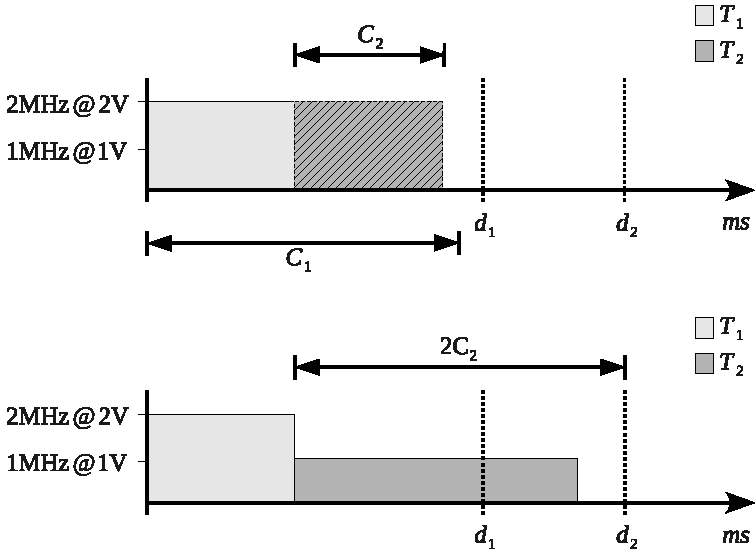
\includegraphics[scale=0.9]{imagens/exemplo-tarefas-usando-dvs.pdf}
        \captionof{figure}{Exemplo de utilização de DVFS em sistemas de tempo real}
        \label{fig:exemplo-tarefas-usando-dvs}
        \end{center}
        \end{figure}
    
    \subsection{Escalonamento em Sistemas RT-DVFS}
        \label{sec:escalonamento-em-sistemas-rt-dvfs}
            
        As primeiras prototipagens de sistemas operacionais embarcados RT-DVFS foram apresentas por \citeonline{Pillai:2001}. Em seu trabalho, foram desenvolvidas heurísticas que, fracamente acopladas ao escalonador do sistema operacional, oferecem consciência energética aos algoritmos \emph{Rate-Monotonic} \cite{Liu:1973} e EDF. \citeonline{Pillai:2001} propõem três classes de heurísticas: as de alteração de tensão estáticas (\emph{Static Voltage Scaling}), as de conservação de ciclos (\emph{Cycle-conserving RT-DVS}) e as de previsão (\emph{Look-ahead RT-DVS}). Das classes citadas, este trabalho utiliza em sua implementação as duas primeiras em conjunto ao algoritmo de escalonamento EDF. Esta escolha é justificada pela simplicidade de implementação e, ao mesmo tempo, por permitir a comparação entre heurísticas que tomam decisões estaticamente e heurísticas que tomam decisões durante a execução do sistema. O funcionamento das duas heurísticas escolhidas é explicado nas seções seguintes.
            
    \subsection{\emph{Static Voltage Scaling} para EDF}
        \label{sec:estaticos}
    
        A primeira abordagem de \citeonline{Pillai:2001} é um mecanismo simples que se beneficia da alteração de tensão e frequência, mantendo a execução das tarefas dentro de seus respectivos prazos. Como o próprio nome da técnica sugere, esta é uma configuração estática da frequência do processador (não se deve confundir com escalonamento estático, como apresentado na seção \ref{sec:escalonadores}). A ideia é obter a menor frequência possível de modo que, mesmo neste baixo desempenho, o conjunto de tarefas satisfaça o teste de escalonabilidade do escalonador EDF. A frequência, por ser configurada estaticamente, só é alterada se o conjunto de tarefas é alterado. Assim sendo, se durante a execução, uma nova tarefa é adicionada ao sistema, o conjunto de tarefas está sendo alterado, então é necessária novamente a escolha de uma nova frequência de funcionamento.
        
        É possível perceber que, alterando a frequência de operação por um fator $\alpha$ $(0 < \alpha \leq 1)$, será necessário alterar os piores tempos de computação para cada tarefa em um fator $1/\alpha$. Observe que os períodos e deadlines, seguindo o modelo apresentando na seção \ref{sec:modelo-de-sistema-de-tempo-real}, mantêm-se inalterados. Com um novo pior tempo de computação, haverá alteração no teste de escalonamento.
        
        % Acrescentar uma figura aqui
        
        Para verificar a escalonabilidade dos conjuntos de tarefas, utiliza-se o teste apresentado na seção \ref{sec:edf}. Este teste, agora com a frequência alterada pelo fator $\alpha$, ficaria como o seguinte\footnotemark:
        
        \footnotetext[1]{O novo teste de escalonabilidade nada mais é do que a aplicação do fator $\frac{1}{\alpha}$ a cada $C_i$ na antiga inequação. Multiplicando os dois lados da inequação por $\alpha$, obtém-se a expressão apresentada aqui.}
        
        Dado um conjunto $T$ de $n$ tarefas $T_i$, para $1 \leq i\leq n$, tais que:
            
   	    \begin{itemize}
	        \item sejam independentes entre si;
	        \item sejam passíveis de preempção;
	        \item sejam periódicas;
	        \item possuam deadlines iguais a seus respectivos períodos.
	    \end{itemize}
       
        $T$ é escalonável por um escalonador EDF se, e somente se $$ \sum_{i=1}^{n} \frac{C_i}{P_i} \leq \alpha.$$
        
        A consciência energética da heurística \emph{Static Voltage Scaling} para EDF consiste então na otimização do conjunto das $m$ frequências possíveis para o processador, sendo escolhida a menor delas capaz de manter o conjunto de tarefas escalonável segundo o teste apresentado. Assim, escreve-se o procedimento \emph{seleciona-frequência}, como expresso no algoritmo \ref{alg:seleciona-frequencia}.
                
        \begin{algorithm}[H]
        \SetKwFunction{testeEDF}{teste-EDF}
        \SetKwFunction{testeRM}{teste-RM}
        \SetKwFunction{seleciona}{seleciona-frequência}
        \SetKwBlock{bloco}{}{}

        \testeEDF{$\alpha$}:
        \bloco{
           \eSe {$\sum_{i=1}^{n} \frac{C_i}{P_i} \leq \alpha$}
                { \Retorna{verdadeiro} }
           { \Retorna{falso} }
        }

        \seleciona:
        \bloco{
            use a menor frequência $f_i \in \left\{f_1,\ldots,f_m|f_1 < \cdots < f_m\right\}$\\
            tal que \testeEDF{$f_i/f_m$} retorne verdadeiro.
        }

        \label{alg:seleciona-frequencia}
        \caption{Alteração estática de tensão para EDF}
        \end{algorithm}
       
        Se o conjunto de tarefas passa no teste de escalonabilidade para a nova frequência e, ainda, as tarefas também não ultrapassam seu novo pior caso de resposta, este mecanismo assegura que os deadlines não serão comprometidos. Se o teste de escalonabilidade falha para todas configurações possíveis, então não é possível escalonar o conjunto de tarefas.
        
        Pela seleção da frequência ser realizada anteriormente à execução do conjunto de tarefas, o novo algoritmo torna-se fracamente acoplado ao escalonador de tempo real \cite{Pillai:2001}, ou seja, uma prévia configuração do sistema pode ser feita, então um escalonador EDF comum pode realizar seu trabalho normalmente, sem necessidade desta entidade entrar em contato com a heurística. Por outro lado, este mecanismo não oferece economia de energia nos momentos onde uma tarefa não atinge seu pior tempo de computação, o que pode acontecer em sistemas reais. Para este caso, algoritmos que levam em conta a utilização real da tarefa, como os expostos adiante, conseguem um melhor benefício.
        
        Um exemplo, apresentado na figura \ref{fig:escalonamento-estatico}, pode ser realizado com as tarefas mostradas na tabela \ref{tab:tarefas-exemplo}. Observe que o pior tempo de resposta ($C_i$) está avaliado para a máxima frequência de funcionamento do processador, ou seja, o caso onde $\alpha=1$ (cenário \emph{a} na imagem). Em um conjunto de três configurações possíveis para frequência, a correspondente a $\alpha=0,75$ é a menor delas que ainda mantém o conjunto de tarefas escalonável (cenário \emph{b} na imagem). Para $0,75>\alpha>0$, algumas tarefas podem perder seus prazos de execução, como é o caso no cenário \emph{c} apresentado na figura, onde a tarefa $T_2$ perde seu deadline.
        
        \begin{figure}[h]
    	\centering
	    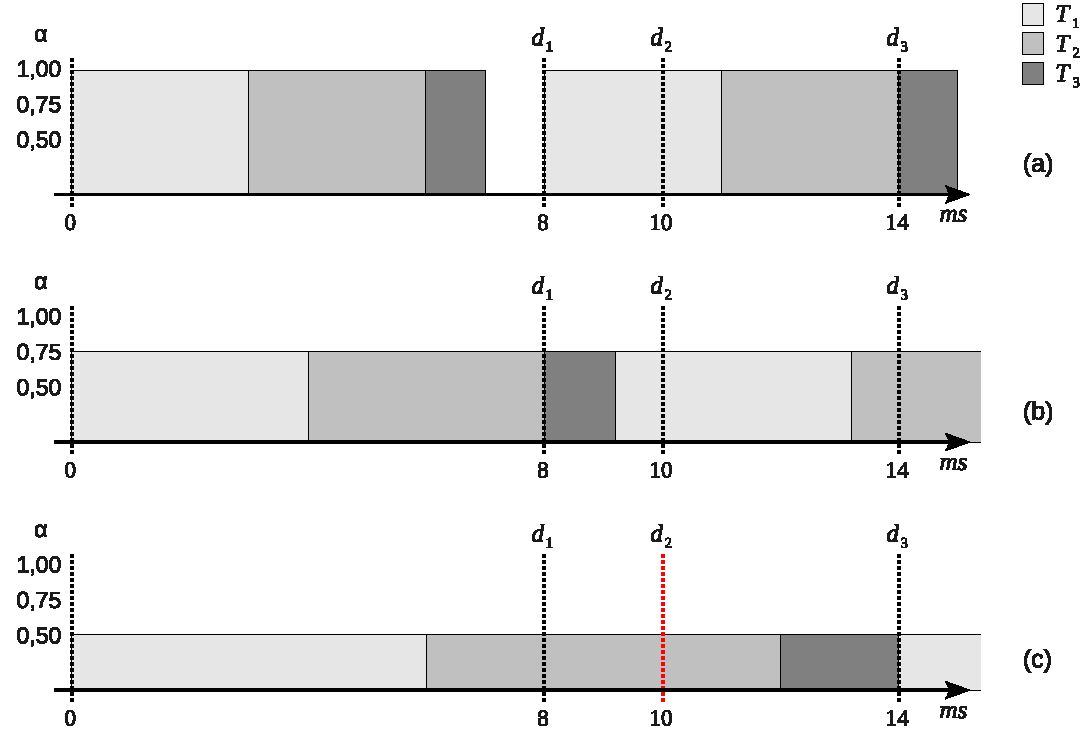
\includegraphics[scale=0.8]{imagens/exemplo-svs-edf.pdf}
    	\caption{Exemplo de escalonamento EDF com alteração estática de frequência}
	    \label{fig:escalonamento-estatico}
        \end{figure}

        \begin{center}
        \begin{table}[h]
        \begin{tabularx}{\textwidth}{ |C|C|C|C| }
            \hline
            Tarefa ($T_i$) &
            Pior Tempo de Computação ($C_i$) &
            Período ($P_i$) &
            Utilização da tarefa ($U_i$)\\ \hline \hline
            
            $T_1$ & $3ms$ & $8ms$ & $0,375$ \\ \hline
            $T_2$ & $3ms$ & $10ms$ & $0,300$ \\ \hline
            $T_3$ & $1ms$ & $14ms$ & $0,071$ \\ \hline
        \end{tabularx}
        \captionof{table}{Exemplo de conjunto de tarefas}
        \label{tab:tarefas-exemplo}
        \end{table}
        \end{center}

        \subsection{\emph{Cycle-conserving RT-DVS} para EDF}
            \label{sec:ccedf}
       
        Uma maneira de tirar maior proveito do uso de DVFS durante o escalonamento EDF é aproveitar as folgas de tempo obtidas quando tarefas não atingem seu pior tempo de computação. De qualquer modo, quando uma tarefa é requisitada para sua execução, não é possível prever o tempo de computação real que será utilizado. Uma solução, proposta por \citeonline{Pillai:2001}, está em assumir que a tarefa inicialmente ocupa seu pior tempo de resposta, mas ao seu término, verificar qual foi o real uso do processador na execução. A ideia desta heurística é então, utilizando estes dados capturados durante a execução das tarefas, adequar o desempenho do processador próximo à utilização real que o conjunto de tarefas promove.
       
        Na heurística \emph{Cycle-conserving RT-DVS} para EDF, três eventos do sistema devem ser capturados: a alteração do conjunto de tarefas, o início da execução de uma tarefa e a conclusão de uma tarefa. A estes eventos, ações são atribuídas:
                      
        \begin{description}
            \item[Na alteração do conjunto] de tarefas, é possível comportar-se como na heurística estática apresentada anteriormente, ou seja, aplicar o algoritmo \ref{alg:seleciona-frequencia} apresentado anteriormente. Isto garante configuração inicial válida para o sistema, sem nenhum prejuízo, já que a heurística \emph{Static Voltage Scaling} é baseada em um cenário de pior caso.
        	\item[No início da execução] da tarefa $T_i$, calcula-se sua utilização no pior caso de computação. Ou seja, assume-se $U_i=C_i/P_i$ até a conclusão da tarefa. Por final, calcula-se a utilização total e aplica-se o algoritmo \ref{alg:seleciona-frequencia} para a seleção da configuração desejada.
        	\item[Na conclusão] da tarefa $T_i$, calcula-se também sua utilização, mas baseando-se agora em seu tempo de computação real $cc_i$. Ou seja, assume-se $U_i=cc_i/P_i$ até que haja uma nova requisição para a tarefa. Novamente, com a utilização calculada, aplica-se o algoritmo \ref{alg:seleciona-frequencia} para a seleção da configuração desejada.
        \end{description}
        
        % Conferir esse exemplo: ver se a tabela de invocações corresponde à execução com alpha = 1.
        
        A figura \ref{fig:cc-edf} demonstra a heurística \emph{Cycle-conserving RT-DVS} para EDF sendo aplicada. O conjunto de tarefas da tabela \ref{tab:tarefas-exemplo} é utilizado como exemplo. A tabela \ref{tab:invocacoes} mostra o tempo de resposta destas tarefas com $\alpha=1$, para a primeira e segunda invocação de cada tarefa. As setas apontam a utilização total calculada no início da execução da tarefa (utilizando-se dados estáticos), e também a utilização total calculada com os dados obtidos \textit{online}, ao final da execução das tarefas.
        
        \begin{figure}[ht]
    	\centering
	    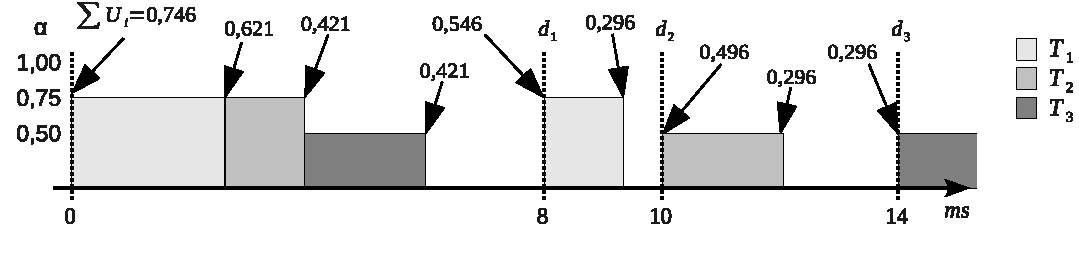
\includegraphics[scale=0.8]{imagens/exemplo-cc-edf.pdf}
    	\caption{Exemplo de escalonamento \emph{Cycle-conserving RT-DVS} para EDF com a utilização calculada em cada início e término de tarefa}
	    \label{fig:cc-edf}
        \end{figure}
        
        \begin{center}
        \begin{table}[ht]
        \begin{tabularx}{\textwidth}{ |C|C|C| }
            \hline
            Tarefa &
            Tempo de Computação na Primeira Invocação &
            Tempo de Computação na Segunda Invocação \\ \hline \hline
            
            $T_1$ & 2$ms$ & 1$ms$ \\ \hline
            $T_2$ & 1$ms$ & 1$ms$ \\ \hline
            $T_3$ & 1$ms$ & 1$ms$ \\ \hline

        \end{tabularx}
        \captionof{table}{Tempo de computação para cada invocação do exemplo}
        \label{tab:invocacoes}
        \end{table}
        \end{center}        
        
        O algoritmo \ref{alg:cc-edf} representa o comportamento da heurística \emph{Cycle-conserving RT-DVS} para EDF. Os procedimentos \emph{tarefa-requisitada} e \emph{tarefa-concluída} são executados em seus respectivos eventos para uma dada tarefa $T_i$. A cada alteração do conjunto de tarefas, \emph{seleciona-frequência} (algoritmo \ref{alg:seleciona-frequencia}) é chamado. Observe que este algoritmo necessita do dado $cc_i$, que é o tempo de computação real utilizado pela tarefa $T_i$. Este é um dado que deve ser calculado em tempo de execução pelo sistema operacional, e além disso, disponibilizado na interface de programação oferecida para a implementação das heurísticas.
        
        \begin{algorithm}[H]
        \SetKwFunction{tarefarequisitada}{tarefa-requisitada}
        \SetKwFunction{tarefaterminada}{tarefa-concluída}
        \SetKwFunction{seleciona}{seleciona-frequência}
        \SetKwBlock{bloco}{}{}

        \seleciona:
        \bloco{
            use a menor frequência $f_i \in \left\{f_1,\ldots,f_m|f_1 < \cdots < f_m\right\}$\\
            tal que $U_1+\cdots+U_n \leq f_i/f_m$.
        }
        
        \tarefarequisitada{$T_i$}:
        \bloco{
           $U_i \leftarrow C_i/P_i$\\
           \seleciona
        }
           
        \tarefaterminada{$T_i$}:
        \bloco{
           $U_i \leftarrow cc_i/P_i$\\
           \seleciona
        }

        \label{alg:cc-edf}
        \caption{\emph{Cycle-conserving RT-DVS} para escalonador EDF}
        \end{algorithm}     
       
       

